\chapter{Modelling Experiments with SCPs} \label{chp:model}
\section{Overview}
As with any cognitive framework, the most important metric for judging the success of SCPs comes from testing how well SCPs can approximate empirical data across tasks. This chapter will show the suitability of SCPs with a common set of allowable cognitive operations for modelling several well-studied experiments in cognitive modelling.

In particular, we will show that the Wason Selection Task, Suppression Task and @TODO can be modelled at both the general and individual reasoner level with SCPs in a formulation that intuitive and consistent with the WCS approach already described in Section~@TODOref.
\section{Suppression Task} \label{sec:supSCP}



To model this experiment in the SCP framework, we must first define the SCP Task $\Pi_{sup}=(s_i,M,f(),\gamma)$ which outlines the restrictions and goals of the model. The structure of $s_i$ must be robust enough to capture information regarding a set of rules, variable assignments in the possible world, and conditionals. To this end we define:

\[s_i^\text{el},s_i^\text{elo}\]
\[s_i^\text{el}=\{S,\Delta_\text{noSup}, V\} \]
\[s_i^\text{elo}=\{S,\Delta_\text{Sup}, V\} \]




For the the only unconditional rule, that she has an essay to write, we define $S=\{(e \leftarrow \top)\}$. The set of conditional rules $\Delta_{\text{noSup}}=\{l|e\}$ captures the probable assumption that she will study late in the library if she has an essay to write, $\Delta_{\text{sup}}=\{(l|e),(l|o)\}$ captures the addition of the conditional that if the library is open she will study late in the library. And the possible world $V=\{(e,u),(l,u),(o,u)\}$ sets all variable names occurring in $S$ and $\delta$ to unknown.

The second consideration $M$, denotes the set of possible cognitive operations which may occur in the resulting SCPs and realised SCPs of $\Pi_{sup}$. Following the intuition we used in Section~@TODOref we choose cognitive operations that enable application of the WCS and interpretation of conditionals. To that end we define:

\[
M=\{\texttt{addAB}, \texttt{semantic}, \texttt{wc}\}
\]

The external evaluation function should translate the SCP into a decision that can be compared with empirical data. In the Suppression Task we will treat $f_\text{sup}()$ as a function that makes a single choice from the set $\{\text{`she will strudy late in the library'},\text{she will not study late in the library}, \text{we are uncertain if she will study late in the library}\}$. Under the assumption only the final state point $p_n$
determines whether she will study late, we might define $f_\text{sup}()$ as follows:

\begin{algorithm}[H] \label{evaluation:f_sup}
\SetAlgoLined
\SetKwProg{Fn}{Function}{ is}{end}
\Fn{$\texttt{f}_\text{sup}(\pi)$}
{
\tcc{This is a final state evaluation SCP.}
Let $R=[(K[\pi],f())]$ be the set of realised SCPs $r_i=(k,f())$ which can be generated from $\pi$\;
Let $P=[\bar{p}_1,...,\bar{p}_n]$, where $\bar{p}_i$ is the final state of $r_i$\;

$P_\text{el}:=[\bar{p} \in P | \bar{p}[\text{`name'}]=\text{`el'}$\;
$P_\text{elo}:=[\bar{p} \in P | \bar{p}[\text{`name'}]=\text{`elo'}$\;

\uIf {there is a response $\in \texttt{responses}(P_\text{el})$ which is not $\in \texttt{responses}(P_\text{elo})$}
{
\Return 'suppression observed'
}
\Else
{
\Return 'no suppression'
}
}
\Fn{$\texttt{responses}(p)$}
{
\Return $[\texttt{response}(\bar{p}) | \bar{p} \in p]$
}
\Fn{$\texttt{response}(\bar{p})$}
{
\uIf{$I_{\bar{p}(V)}(l)\models \top$}
{
\Return `she will study late in the library'
}
\uElseIf{$I_{\bar{p}(V)}(l)\models \bot$}
{
}
\Else
{
\Return `we are uncertain if she will study late'
}
}

\caption{$\texttt{f}_\text{sup}$}
\end{algorithm}

It is worth noting that one could also define $f_\text{sup}$ in such a way that it iterates over every variable assignment for 'el' and 'elo' in the final state point and sees if any inference is drawn in 'el' that is not drawn in 'elo'. However, the purpose of the external evaluation function is to transform an SCP into an output from the set of empirically observed outputs, and in this case the empirical knowledge is a response to the question ``will she study late in the library?".

Next, we define the empirical result we wish to emulate $\gamma$. In this case we will define $\gamma_{text{noSup}}$ to model cases where no suppression is observed, and $\gamma_{\text{sup}}$ to model cases where suppression is observed.

\[\gamma_{\text{noSup}} = \text{no suppression} \]
\[\gamma_{\text{sup}} = \text{suppression observed} \]

Armed with these definitions, it is possible to model the task $\Pi$ as follows:

\[\Pi=(s_i,M,f(),\gamma_{\text{sup}})\]

De Novo search on $\Pi$ returns the satisfying SCP $\mu_\text{sup}$:

\[\mu_\text{sup}=(\pi=(s_i \longmapsto \texttt{addAB} \longmapsto \texttt{wc} \longmapsto \texttt{semantic}),f())\]

Figure~\ref{fig:Suppression_SCP} illustrates the realised SCP for $\mu_\text{sup}$ and illustrates that $\mu_\text{noSup} \models \gamma$. This example has served to show that suppression can modelled in the SCP framework.

\begin{figure}
\centering 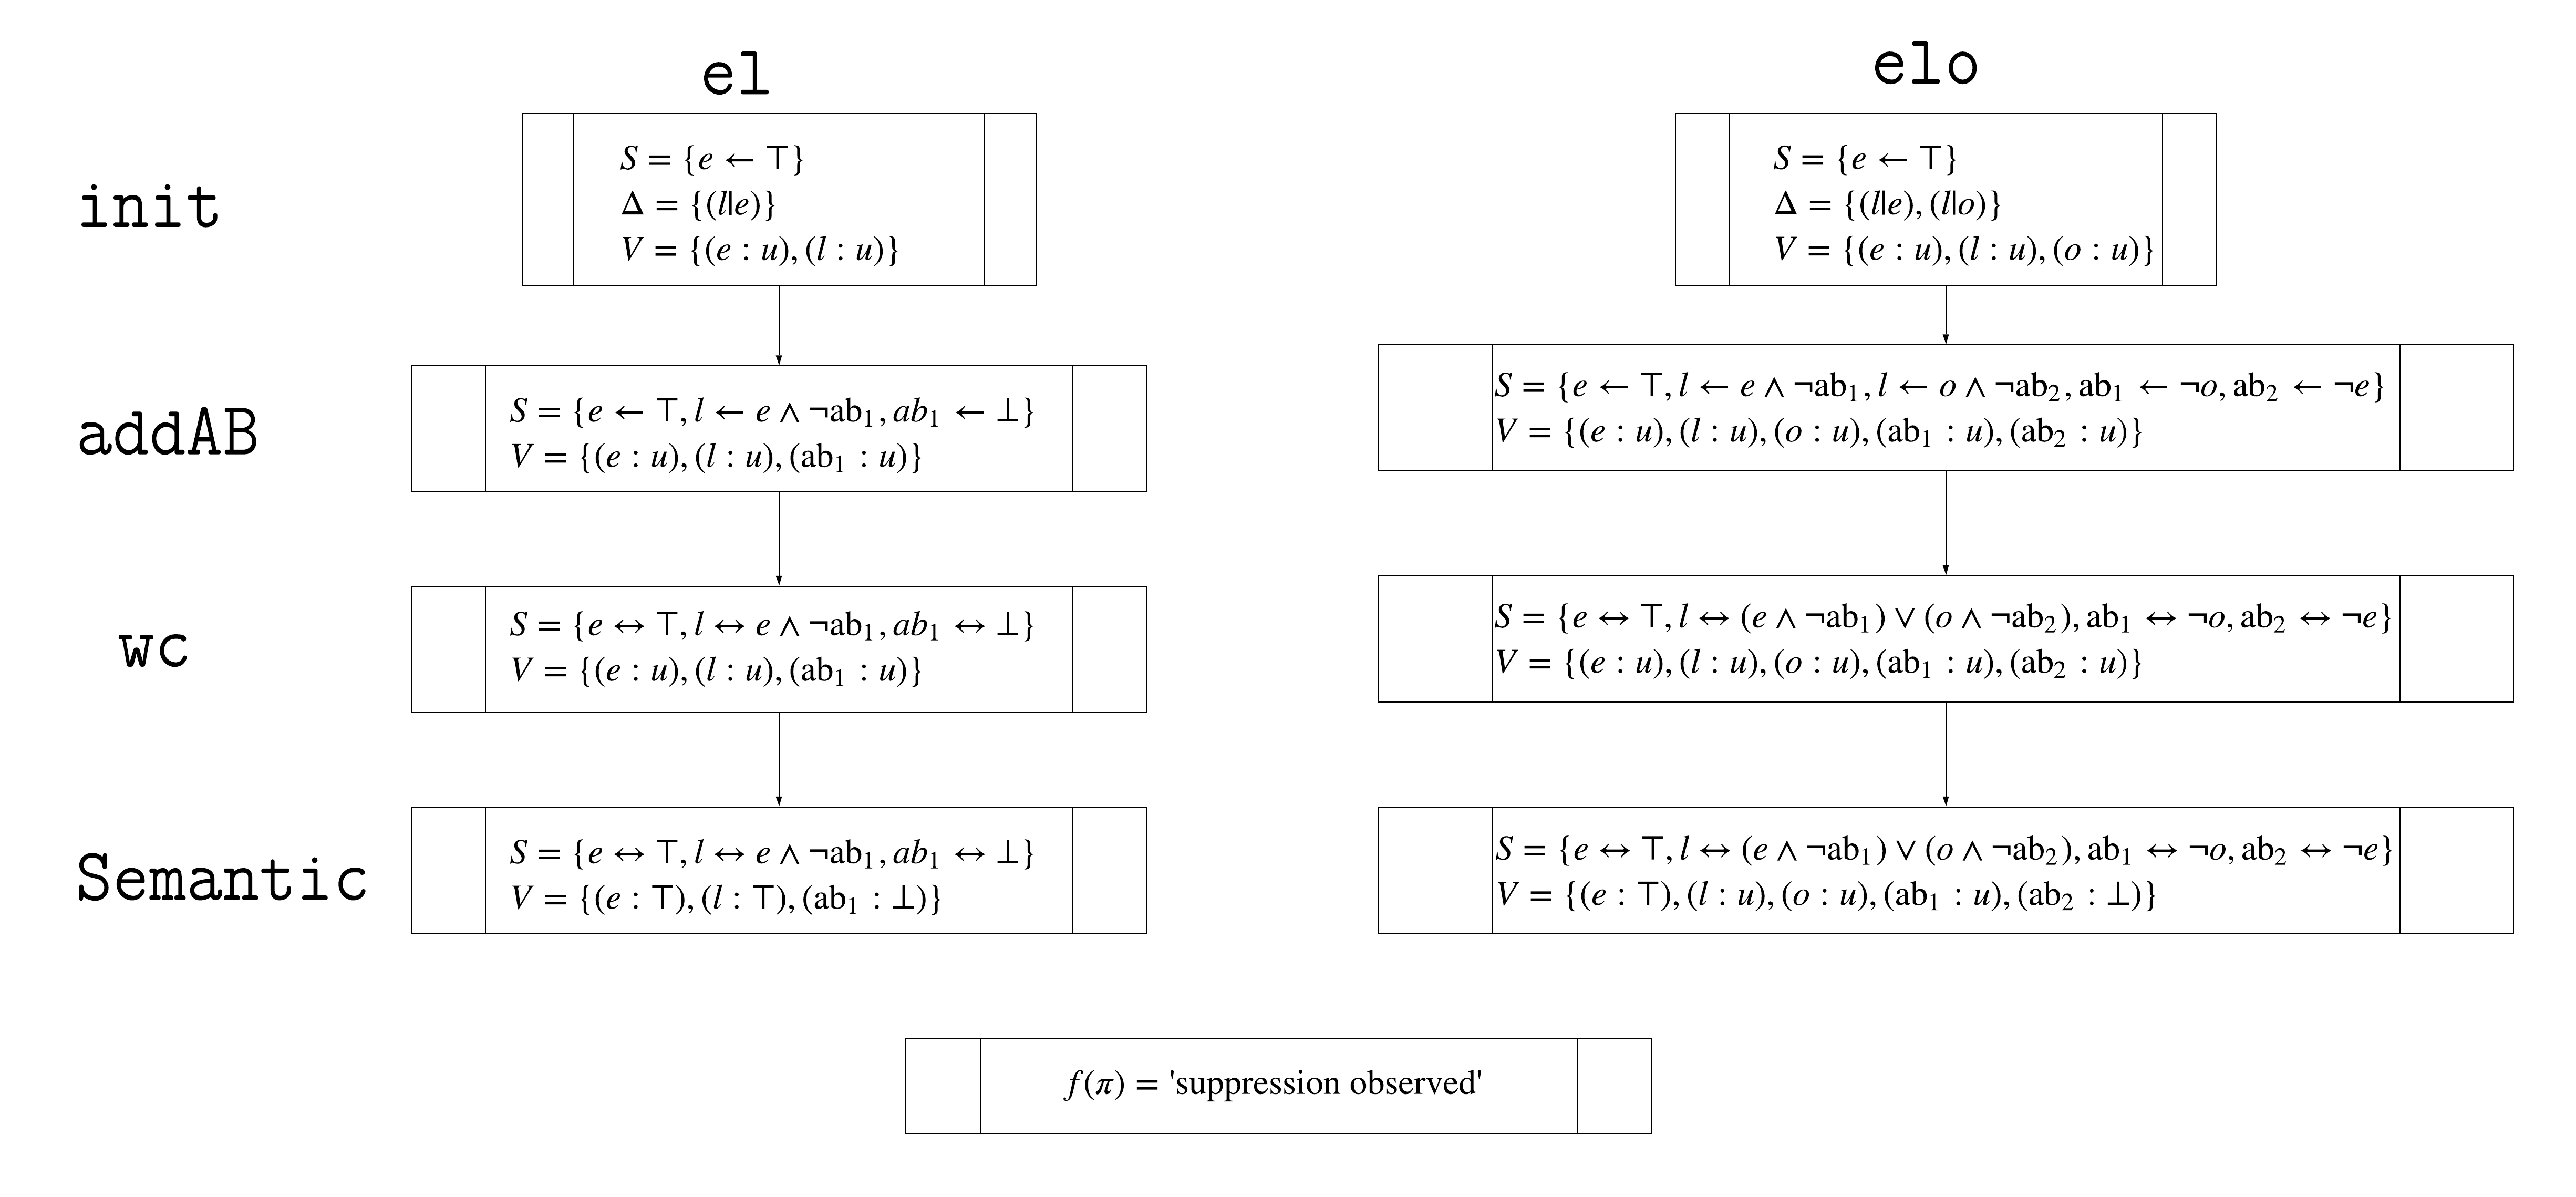
\includegraphics[scale=0.4]{Suppression_SCP}
\caption{Suppression for the two SCPs $\mu_\text{noSup}$ and $\mu_\text{sup}$}.
\label{fig:Suppression_SCP}
\end{figure}

%==========================individual reasoners===================================

To illustrate the ability of the framework to model individual reasoners, we examine those reasoners who despite knowing both that if she has an essay to write she will study late in the library and that if the library is open she will study late in the library still do not demonstrate suppression, and instead draw the classical conclusion that she will study late in the library. To this end we define a second SCP Task $\Pi_\text{deviant}$.

\[\Pi_\text{deviant}=(s_i^{\text{sup}},M',f(),\gamma_{\text{noSup}})\]
\[M'=\{\texttt{addAB}, \texttt{semantic}, \texttt{wc}, \texttt{remove}_\bot, \texttt{addExp}\}\]

$M'$ is contains $\texttt{remove}_\bot$ which is able to delete any subset of the variables mentioned in $R[\text{`delete'}]$ of the epistemic state. $\texttt{addExp}$ allows us to add abducible facts to an epistemic state, following the intuition we used to model the WST (@TODORef). To see the explanations and justifications for these two cognitive operations, refer to Section~\ref{ssec:deletion}, and Section~\ref{ssec:abd}.

Equipped with these two cognitive operations, there are several SCPs which can model $\Pi_\text{deviant}$.

Figure~\ref{fig:Suppression_SCP_del1} shows the realised SCPs for one satisfying SCP for $\Pi_\text{deviant}$. This example shows that deleting the variable $o$ from the epistemic state, prevents suppression from occurring because suppression the abnormality $(\text{ab}_1 \leftarrow \lnot o )$ is the cause of the suppression in $\Pi$, and in $\Pi'$ the abnormality is now given by $(\text{ab}_1 \leftarrow \lnot \top )$.

Appendix~@TODOref shows that the non-monotonic cognitive operation \texttt{addExp} can prevent suppression by adding abducibles related to the  free variable $o$.\footnote{The output is too large to graph attractively, and should be viewed in its entirety to confirm that this approach is effective.} This is, as far as I can tell, the first use of @TODOs abducible approach to the WST to model the Suppression Task. By giving $o$ an assignment, the abnormality $\text{ab}_1\leftrightarrow \lnot o$ no longer evaluates to $u$, and across all responses epistemic states, the `elo' states now model every response \texttt{response} that `el' does.

Both of these examples illustrate the derivation of the classical logical response to the suppression task as a modification of an SCP which did illustrate suppression. This evidences one of the core claims of the SCP Framework which is that it is a reasonable tool for modelling individual reasoners in a cognitive task. 

The value of these examples lies in that they show that classical logic response to a cognitive task is not necessarily derived through the use of classical logic.

\begin{figure}
\centering 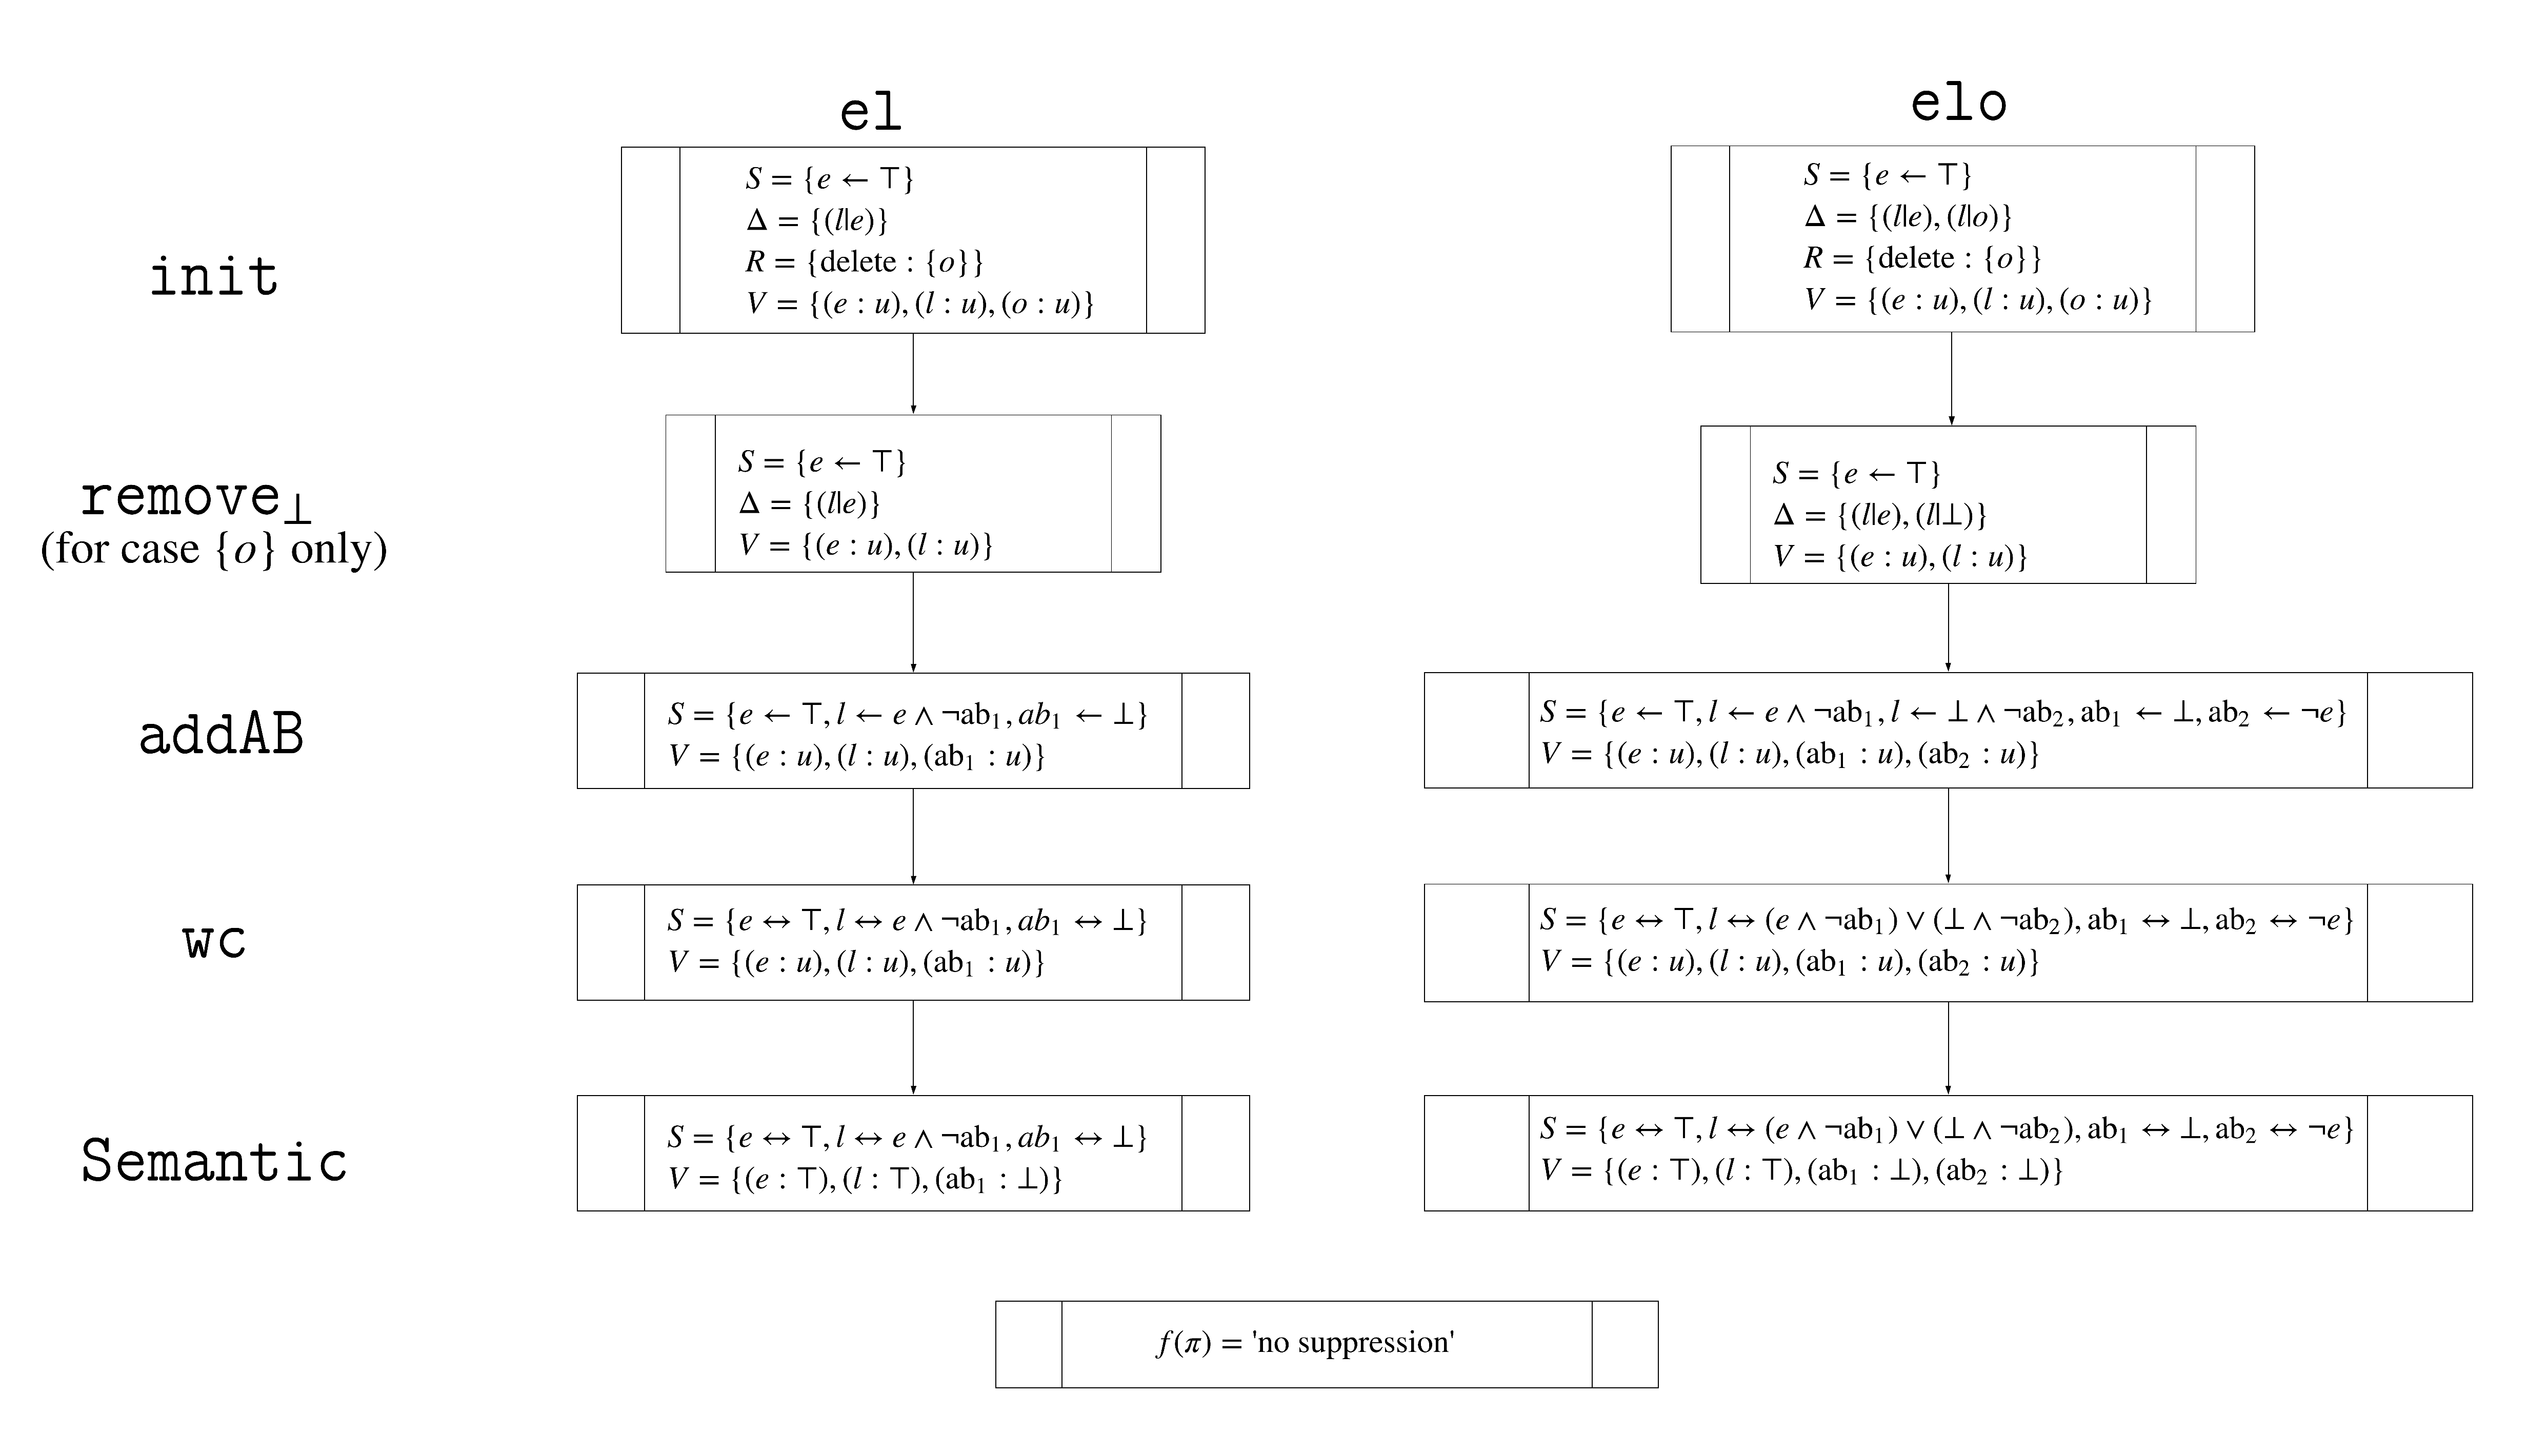
\includegraphics[scale=0.4]{Suppression_SCP_del1}
\caption{Inhibition of Suppression for the SCP $\mu_del=(\pi,f_\text{sup}()), \pi = (s_i \longmapsto \texttt{remove}_\bot \longmapsto \texttt{addAB} \longmapsto \texttt{wc} \longmapsto \texttt{semantic}).$}.
\label{fig:Suppression_SCP_del1}
\end{figure}


\section{Wason Selection Task}\label{sec:wstSCP}

We define the SCP Task $\Pi=(s_i,M,f(),\gamma)$ to model the WST. The choice of external evaluation function for this task (the turn function), if we are to follow the intuition from Section~\ref{ssec:sup_mod}, has two requirements: it must be able to capture whether an observation $O$ can be explained by the least model of the weakly completed program, and it must ensure that variable assignments which could falsify or verify the conditional rule $(3|D)$, are present in the least model. 

To this end, we add an observation variable $O$ to the definition of turn function, and combine this with the variables for the set of propositional rules $S$, conditional rules $\Delta$, and possible world $V$.

Next, we require an intuition for the generation of the initial epistemic state point $s_i$. In this case, abduction can be simulated by the SCP in one of three ways. The first is to create a unique SCP for each possible explanation for each observation as we did for the classical WCS interpretation of the task in Section~\ref{ssec:sup_mod}. But the fact that SCPs may contain an initial state point, rather than just a single epistemic state, enables a more elegant solution that captures the full scope of possible observation, explanation pairings. The other two options are to start with a state point containing each abductive case, or to create cognitive operations which create these abductive cases at computation time.

Because SCPs aim to capture as much cognitive information as possible within the CTM as possible, we will prefer this third case and make use of the categorization variable $R$ to specify both the set of observations, and the possible explanations. The cognitive operation \texttt{AddExp} is created.

In a significant alteration to the logic we followed with the WCS approach to the WST, we will create a single SCP to model the turn function for each card. Our initial state for this for this task will contain the initial conditional rule, no propositional rules, and will make use of the categorization variable $R=\{\text{explanations}\}$ to store information about the producible which may added to the epistemic state at some time point. With this in mind we define:

\[
s_i=(S,\Delta, R)
\]
\[
S=\{\}
\]
\[
\Delta=\{(3|D)\}
\]
\[
R=\{\text{explanations}:\{D\leftarrow \top, D \leftarrow \bot, K\leftarrow \top, K \leftarrow \bot, 3\leftarrow \top, 3 \leftarrow \bot, 7\leftarrow \top, 7\leftarrow \bot\}\}
\]

For the purposes of readability, we will restrict examination of the abducibles to cases that are of length 1, and contain only positive facts\footnote{A reader wishing to see this process with respect to the full set of abducibles should examine the \texttt{WST.py} file in the SCP implementation.}.

Next, we define the external evaluation function $f_\text{wcs}(\pi)$ as follows:

\begin{algorithm}[H] \label{cogOp:wcs}
\SetAlgoLined
\SetKwProg{Fn}{Function}{ is}{end}
\Fn{$\texttt{f}_\text{WST}(\pi)$}
{
\tcc{This is a final state evaluation SCP.}
Let $R=[(K[\pi],f())]$ be the set of realised SCPs $r_i=(k,f())$ which can be generated from $\pi$\;
Let $P=[p_1,...,p_n]$, where $p_i$ is the final state of $r_i$\;
Let $\eta_i=[\eta_1,...,\eta_n]$, where $\eta_i=p_i[R][\eta]$\;
Let $O=\{(D,\top),(K,\top),(3,\top),(7,\top)\}$ be the set of observations\;
Let $C=\{(3|D), (D' | 7)\}$ be the set of conditionals which must be falsified or verified.\;
Output={}\;
\For{$p_i \in P$}
{
run \texttt{isExplanation}($p_i$)\;
}

\For{each minimal explanation $e$ for observation $o$}
{
\uIf {$I_\text{e[{`V'}]}(C)$ either falsifies or verifies some conditional in $C$}
{
Output[o]:=Output[o]$\cup$ `Turn Card'\;
}
\Else
{
Output[o]:=Output[o]$\cup$ `Do not turn Card'\;
}
}

\Return Output
}
\Fn{$\texttt{isExplanation}(\pi)$}
{
\If{$I_{p_i['V']}(p_i['S']) \models (o) \in O$}
{
\tcc{Then $p_i$ explains $o$.}
Add $p_i$ to the explanations for $o$.
}
}

\caption{$\texttt{f}_\text{WST}$}
\end{algorithm}







Figure~@TODOref shows the state point that results from applying this cognitive operation to $s_i=(S=\{\},\Delta=\{(3|D)\},V=\{D,K,3,7\},O=\{\},R=\{'explanations':\{D,K,3,7\}\})$ for cases where $R$ is a single abducible.

Because the intention of this task is to model a known response set for the WST, we must consider some way of generating an SCP in which $f(\pi)\models \gamma$. As before this necessitates an appropriate selection of cognitive functions for $M$. We will make use of the set:

\[
M=\{\texttt{addAB},\texttt{wc},\texttt{semantic}, \texttt{addExp}\}
\]

Conducting de Novo search on $\Pi$ for each of the observations at this point now returns a state point containing the following CTMs:
@TODOwegothereish
\[
\pi_1=(s_i \longmapsto \texttt{addAB} \texttt{addExp} \longmapsto \longmapsto \texttt{wc} \longmapsto \texttt{semantic}))
\]

\[
\pi_2=(s_i \longmapsto \texttt{addExp} \longmapsto \texttt{addAB} \longmapsto \texttt{wc} \longmapsto \texttt{semantic}))
\]


\[
\mu_D^1=(\pi_1), f(\pi, O=\{D\}))
\]
\[
\mu_D^2=(\pi_2), f(\pi, O=\{D\}))
\]

\[
\mu_K^1=(\pi_1), f(\pi, O=\{K\}))
\]
\[
\mu_K^2=(\pi_2), f(\pi, O=\{K\}))
\]

\[
\mu_3^1=(\pi_1), f(\pi, O=\{3\}))
\]
\[
\mu_3^2=(\pi_2), f(\pi, O=\{3\}))
\]

\[
\mu_7^1=(\pi_1), f(\pi, O=\{7\}))
\]
\[
\mu_7^2=(\pi_2), f(\pi, O=\{7\}))
\]

@TODOcontra, indroduce $(3|D) \land (D' | 7 )$ interpretation using de finetti truth table.

\begin{figure}
\centering{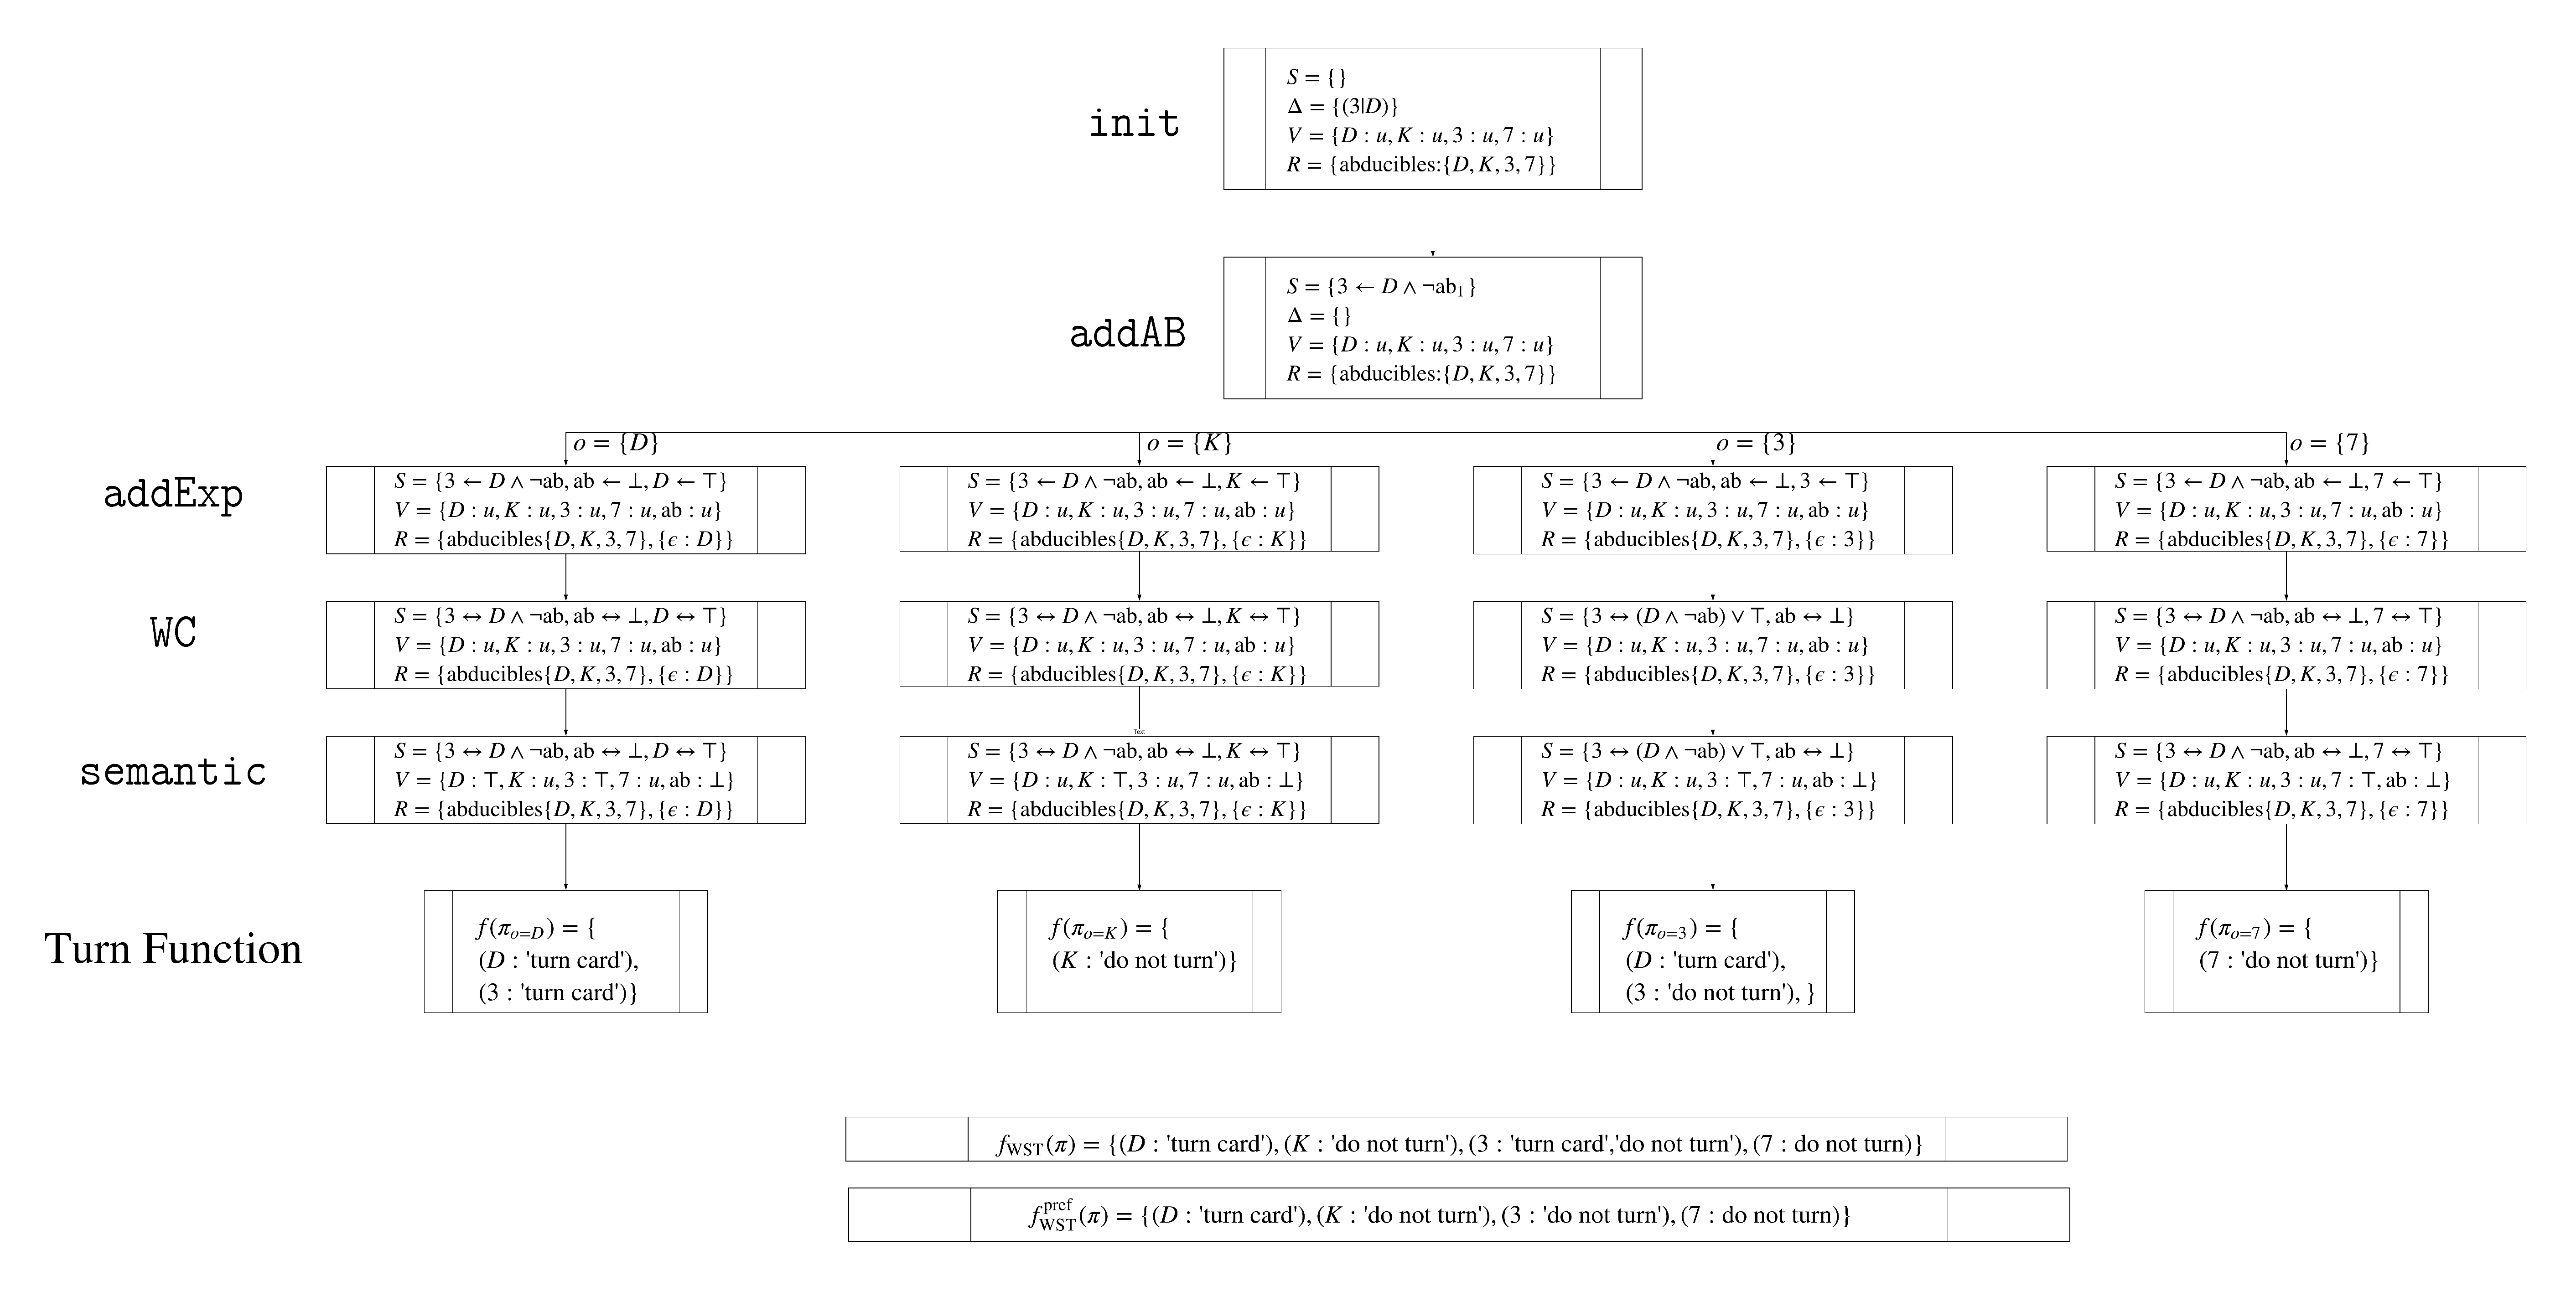
\includegraphics[width=\linewidth]{realisedSCPsWST}}
\label{fig:rSCP_WST}
\caption{Realised SCPs for the SCP interpretation of the WST $\pi_1=(s_i \longmapsto \texttt{addAB} \longmapsto \texttt{addExp}  \longmapsto \texttt{wc} \longmapsto \texttt{semantic}))$. Results mimic those observed in @TODOref's WST interpretation.}
\end{figure}

These results are not surprisingly and illustrate two important points. The first is that, for external evaluation functions that only evaluate the final epistemic state $p_n$, $f(\pi_1,O=\{o\})=f(\pi_2,O=\{o\})$ for any observation $o$. Secondly, the non-monotonic cognitive operation \texttt{addExp} means that these SCPs do not necessarily produce a single base point for $p_n$ and it will be necessary to examine the realised SCPs to determine which cards can actually be turned. Figure~\ref{fig:rSCP_WST} shows the realised SCP that can be produced for explanations of length 1 (as with @TODOcite's original WCS interpretation minimal explanations are preferred) using CTM $\pi_1$. @TODOdefineindependenceofcognitiveoperations. 

\begin{figure}
\centering{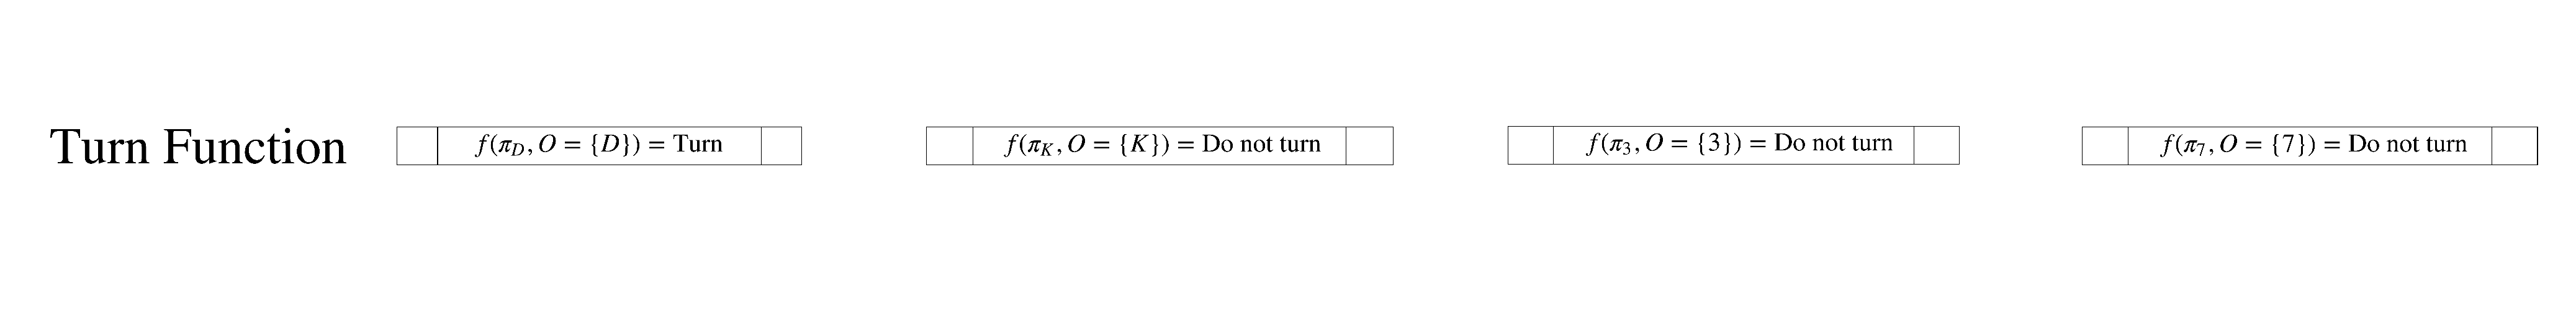
\includegraphics[width=\linewidth]{realisedSCPsWST_simple}}
\label{fig:rSCP_WST_simple}
\caption{Realised SCPs for the simplified SCP interpretation of the WST $\pi_1=(s_i \longmapsto \texttt{addAB} \texttt{addExp} \longmapsto \longmapsto \texttt{wc} \longmapsto \texttt{semantic}))$.}
\end{figure}

In order to model the three deviant cases of WST, we follow the same reasoning discussed in Section~@TODOsec and introduce two extensions to our original model: Basic Weak Completion, and Contraposition.

Basic Weak Completion is achieved by formulating a new external evaluation function $f'(\pi)=f(\pi,O=\epsilon)$. Because $I_V(\top)\models \top$, the observation is trivially satisfied and the evaluation function simply depends on whether the possible world of realised SCP assigns values which, if they were otherwise, could violate the conditional $(3|D)$. Figure~\ref{rSCP_WST_simple} illustrates $f'(r)$ for each of the realised SCPs generated in the abductive interpretation of SCPs, where the explanation $\epsilon$  is minimal.

Contraposition can be achieved by creating a new congitive operation \texttt{contra} which applies add the classical modus tolens implications to all conditionals contained in $\Delta$ of the input state.

%------
\[\texttt{contra}(\textit{input})=(\chi,e)\]
\[\chi=(\textit{input}\models (\Delta))\]
\[\Delta' := \Delta\]
\[\forall_{(\psi|\phi) \in \Delta'}\]:
\begin{itemize}
\item $S:=S \cup (\phi'\leftarrow \lnot \phi)$
\item $\Delta := \Delta\cup (\phi'| \lnot \psi)$
\item $V:=V\cup(\phi':u)$
\end{itemize}
%------



















